\section{Database Design}
Following the modeling of the system’s dynamic behavior through activity diagrams, it is essential to define how data is structured, stored, and managed within the system. 
\subsection{Object-Relational Mapping Rules}

The transformation from the object-oriented model to the relational model is based on the following rules \cite{elmasri2016database,fowler2002patterns}:

\begin{itemize}
	\item Each class is mapped to a table
	\item Each attribute is mapped to a column
	\item The identifier becomes the primary key
	\item Associations are translated into foreign keys
	\item Many-to-many relationships are implemented using junction tables
\end{itemize}

These rules are directly applied based on the class diagram.

\subsection{Relational Schema}

The relational schema of the system is defined as follows:

\begin{itemize}
	\item \textbf{User} (\underline{id}, userName, email, phone, password, isAdmin, isValidated, createdAt)
	
	\item \textbf{Farmer} (\underline{id}, \#user\_id)
	\item \textbf{Buyer} (\underline{id}, address, license\_image, \#user\_id)
	\item \textbf{Transporter} (\underline{id}, region, wilaya, baladiya, driver\_license\_image, \#user\_id)
	\item \textbf{Ministry} (\underline{id}, \#user\_id)
	
	\item \textbf{Farm} (\underline{id}, name, address, baladiya, wilaya, size, \#farmer\_id)
	
	\item \textbf{ProductCategory} (\underline{id}, name, slug, description, isActive)
	
	\item \textbf{Product} (\underline{id}, title, description, unite\_price, quality, stock, inStock, publishedAt, average\_rating, review\_count, \#farm\_id, \#category\_id)
	
	\item \textbf{ProductImage} (\underline{id}, url, altText, \#product\_id)
	
	\item \textbf{Cart} (\underline{id}, \#buyer\_id)
	\item \textbf{CartItem} (\underline{id}, quantity, \#cart\_id, \#product\_id)
	
	\item \textbf{Order} (\underline{id}, status, shippingAddress, orderDate, paymentStatus, \#buyer\_id)
	
	\item \textbf{OrderItem} (\underline{id}, quantity, \#order\_id, \#product\_id)
	
	\item \textbf{Invoice} (\underline{id}, totalAmount, \#order\_id)
	
	\item \textbf{Vehicle} (\underline{id}, type, plateNumber, capacity, model, \#transporter\_id)
	
	\item \textbf{DeliveryMission} (\underline{id}, status, pickupLocation, deliveryLocation, wilaya, assignedAt, deliveredAt, \#order\_id, \#transporter\_id, \#vehicle\_id)
	
	\item \textbf{OfficialPrice} (\underline{id}, minPrice, maxPrice, season, \#ministry\_id, \#category\_id)
\end{itemize}
The following figure presents the relational schema of the system, illustrating the different tables and the relationships between them.
\begin{figure}[H]
	\centering
	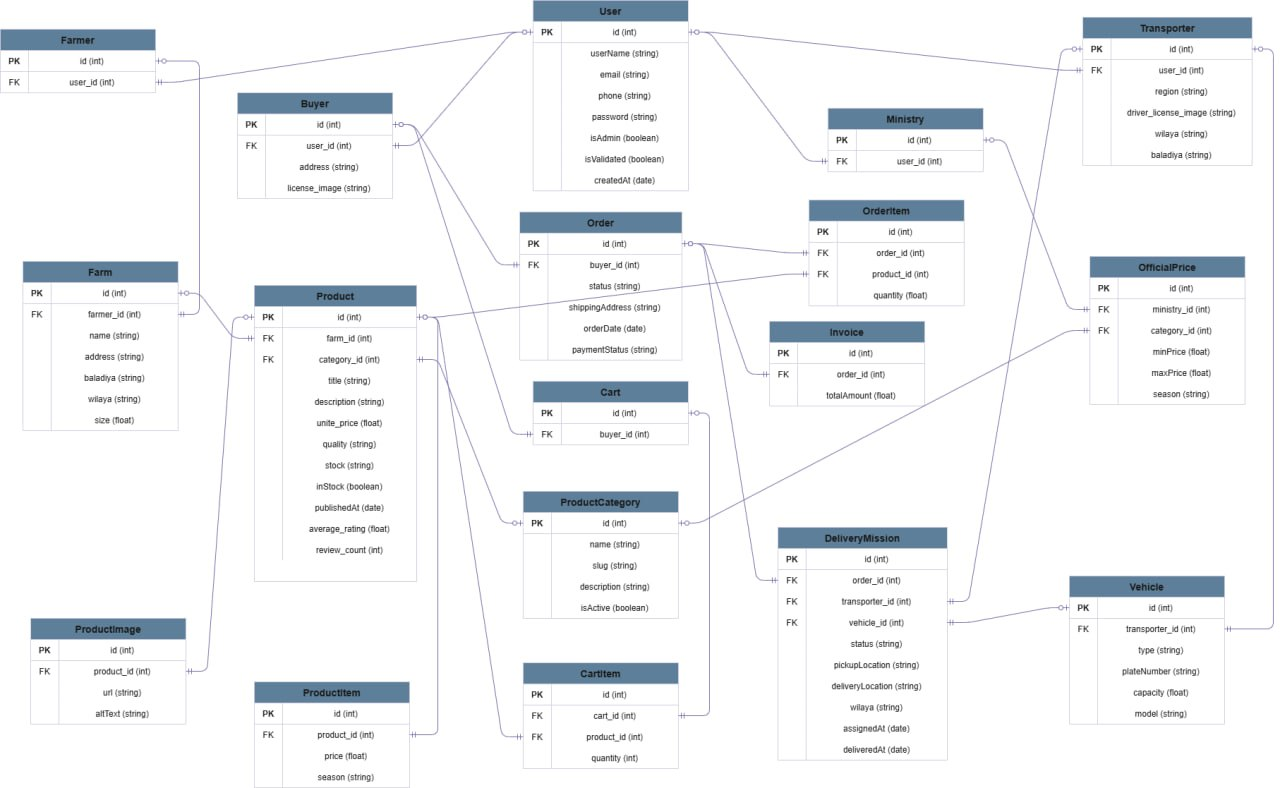
\includegraphics[width=1.1\linewidth]{images/diagrammes/schema_relationnel}
	\caption{Relational Schema}
\end{figure}

This schema is directly derived from the design class diagram and reflects the system’s data structure and relationships between its main entities.